\section{Debian Server}
\subsection{Allgemeine Sachen}
\begin{itemize}
\item \textbf{Benutzer:} BN:debian PW:debian (Settings änderbar in GNS3)
\end{itemize}
\subsection{DHCP}
\textit{\textbf{Aufgabenstellung:} Stelle ein, dass eine fixe MAC-Adresse immer die gleiche IP zugewiesen bekommt}

\begin{itemize}
\item \textbf{Superuser Rechte}
\begin{verbatim}
sudo su
\end{verbatim}

\item Öffne die DHCP-Config file auf dem Debian Server, schreibe folgende Zeilen in die File
\begin{verbatim}
vi /etc/network/interfaces
\end{verbatim}

\item \textbf{DHCP Aktivieren}
\begin{verbatim}
# DHCP config for ens4
auto ens4				## Change
iface ens4 inet dhcp		## Change
\end{verbatim}

\item \textbf{Netzwerk Schnittstelle Neustarten}
\begin{verbatim}
systemctl restart networking	## Wenn im ROOT
sudo systemctl restart networking ## Wenn nicht im ROOT
\end{verbatim}
\end{itemize}

\newpage

\subsection{lighttpd auf Debian installieren}
\begin{itemize}
\item Linux aktualisieren
\begin{verbatim}
$ sudo apt update
$ sudo apt upgrade
\end{verbatim}

\item lighttpd Installieren
\begin{verbatim}
$ sudo apt install lighttpd
\end{verbatim}

\item mit curl kann man prüfen ob system läuft (wenn nicht installiert "\$ sudo apt install curl" installieren\\ IP vom Debian Server 192.168.3.76 \\ IP von außen auf den Router: 192.168.122.254
\begin{verbatim}
curl 192.168.122.254
\end{verbatim}

\item auf Browser IP vom Router außen (192.168.122.254) zugreifen $\rightarrow$ kommt man zu der Placholder page von 192.168.122.254
\end{itemize}

\newpage

\subsubsection{Host Laptop auf Debian Server zugreifen}
\textit{\textbf{Problemstellung:} Wie kann ich von außen auf dem Server zugreifen?}\\
\textbf{Problem:} Wenn ich auf die $192.168.3.76$ von außen auf dem Router zugreifen will, geht das nicht, da der Router keine interne Verbindung von Außen nach Innen hat. Deswegen brauchen wir eine Forwarding Rule der Firewall die das einfach weiterleitet. Wenn man die lighttpd Standard-Einstellungen lässt, läuft der Server auf Port 80 (http), was in die Firewall-Rule reingehört. Von Außen lässt sich der Router nicht auf $192.168.3.1$ zugreifen und muss über $ip a$ die IP meines Router von Host PC rausfinden. Damit lässt sich der Router von außen Pingen. Den Debian Server kann ich nicht darüber Pingen, da Ping ein Port ist. Aber mit curl lässt sich der Quellcode von Port 80 anschauen.

\begin{figure} [!ht]
	\centering
	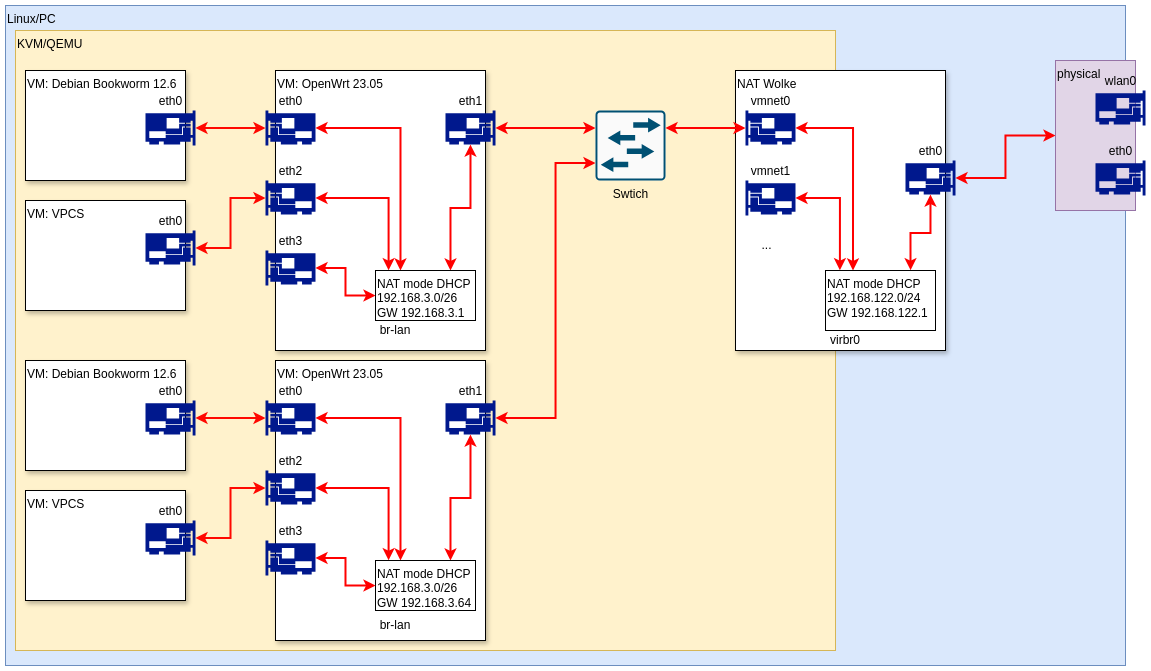
\includegraphics[width=1\textwidth]{images/Aufbau.png}
	\caption{Blockschaltbild für Beispiel}
\end{figure}

\end{itemize}